% \chapter{DATA COLLECTION, ANALYSIS AND RESULTS}

\begin{sloppypar}
	
	\section{Original Dataset}
	For this study, data obtained were through interviews with student residents in the hostels.
	The dataset is a cleaned dataset from 495 responses from 70 distinct hostels (Table \ref{table:2}).
	Since most hostels can be located in Ayeduase and Kotei, 38 and 20 hostels were selected from Ayeduase and Kotei, respectively, and 6 each from Bomso and Kentinkrono.

		\begin{longtable}{p{3cm}p{3cm}p{7cm}}
			\caption{Features Description} 
			\label{table:1} \\
			\hline
			\textbf{Name} & \textbf{Type} & \textbf{Description} \\ \hline
			location & categorical & general location of hostel \\ %\hline
			grade & numerical & average of students' evaluation \\ %\hline
			rank & categorical & overall quality of hostel \\ %\hline
			beds & numerical & beds in a room \\ %\hline
			study room & categorical & hostel's study room \\ %\hline
			tv room & categorical & hostel's tv room \\ %\hline
			security & categorical & security personnel or post \\ %\hline
			food joint & categorical & food joint within 5 minutes walk \\ %\hline
			external power & categorical & another source of power \\ %\hline
			ac & categorical & air conditioner in a room \\ %\hline
			proximity & numerical & distance to \ac{cos} \\ %\hline
			post code & categorical & post code of hostel \\ %\hline
			latitude & numerical & hostel's latitude \\ %\hline
			longitude & numerical & hostel's longitude \\ %\hline
			price2018 & numerical & price of room for 2018/19 in cedis \\ %\hline
			price2019 & numerical & price of room for 2019/20 in cedis \\ %\hline
			price2020 & numerical & price of room for 2020/21 in cedis (target feature) \\ \hline
		\end{longtable}
	
	
	\section{Results}
	First, we check the assumption of \ac{mlr} model. Figure \ref{fig:var} shows no notable patterns in our residuals and a negligible correlation; hence, equality of variance and independence of observation assumptions are met. Figure \ref{fig:norm} shows a plot with data points close to the normal line; a t-test on the residuals produced a p-value of $ >> 0.05 $; as a result, the normality assumption can be accepted. Since all assumptions are met, the \ac{mlr} model qualifies as a candidate model for our dataset.
	\vspace*{0.5cm}
	
	\begin{figure}[h]
		\centering
		\begin{subfigure}[h]{0.47\textwidth}
			\centering
			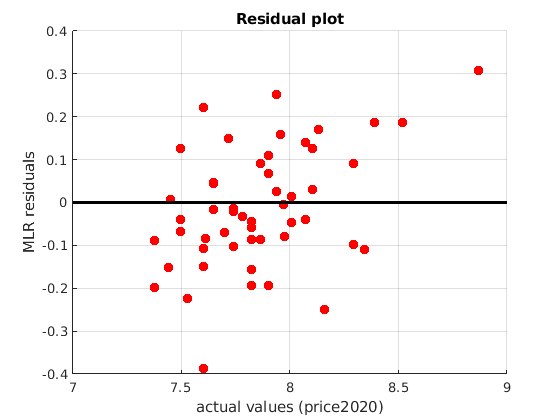
\includegraphics[width=\textwidth]{lmres}
			\caption{Equality of Variance}
			\label{fig:var}
		\end{subfigure}
		\hfill
		\begin{subfigure}[h]{0.47\textwidth}
			\centering
			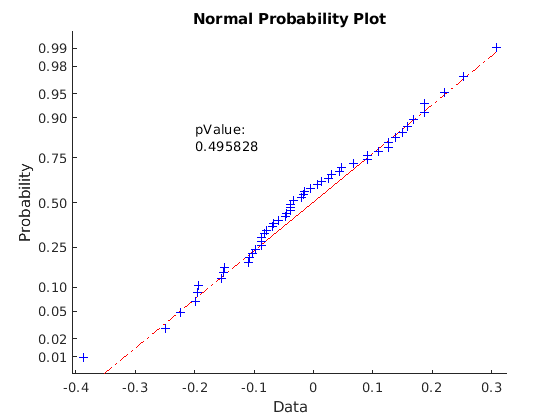
\includegraphics[width=\textwidth]{lmprob}
			\caption{Normality of Residuals}
			\label{fig:norm}
		\end{subfigure}
		\caption{Analysis of Residuals}
		\label{fig:allerr}
	\end{figure}
	
	\hspace*{-0.6cm}The evaluation metrics given by equations \ref{eqn:mae}, \ref{eqn:rmse} and \ref{eqn:r2} of both train and test sets are presented in Table \ref{table:metric}
	
	\begin{table}[h!]
		\centering
		\caption{Evaluation Metrics of Train and Test sets}
		\label{table:metric}
		\begin{tabular}{|c|p{1.5cm}p{1.5cm}c|p{1.5cm}p{1.5cm}c|}
			\hline
			\multirow{2}{*}{MODELS} & \multicolumn{3}{|c|}{TRAIN SET} & \multicolumn{3}{|c|}{TEST SET} \\ \cline{2-7}
			& MAE & RMSE & $R^2$ & MAE & RMSE & $R^2$ \\ \hline
			\ac{mlr} & 0.1069 & 0.1337 & 0.7968 & 0.1114 & 0.1382 & 0.79 \\
			\ac{rr} & 0.1142 & 0.1406 & 0.7753 & 0.1116 & 0.1443 & 0.7711 \\
			\ac{nn} & 0.1069 & 0.1337 & 0.7968 & 0.1125 & 0.1398 & 0.7852 \\ \hline
		\end{tabular}
	\end{table} 
	
	\hspace*{-0.6cm}From Table \ref{table:metric}, all three models performed well, with all coefficients of determination of the test set close to 1. However, the \ac{rr} which was implemented to improve the fit in \ac{mlr} utilizing its embedded feature selection properties with lambda of 0.0103, produced an $ R^2 $ lesser than the \ac{mlr} model. Moreover, the \ac{mlr} generalized well on the test set with an $ R^2 $ of 0.79; this could be as a result of no or negligible over-fitting and/or issues of collinearity. \newline
	The \ac{nn} modeled the relationship between predictors and target features with two layers - a hidden layer with 10 nodes and an output layer with 1 node. The model, as noted by \citep{Phan2019}, works like a "black box," and we do not know the relationship between the predictors and the price prediction. Even so, the model performed exactly as \ac{mlr} model on the train set. However, on the test set, there was a reduction in all three evaluation metrics (Figure \ref{table:metric}).
	\newpage  
	\hspace*{-0.6cm}Using the same models developed by our machine learning algorithms by learning from the entire dataset, we will explore the existence of submarkets \citep{maclennan1996economic} in the AYEDUASE and KOTEI areas using the table below.
	
	\begin{table}[h!]
		\centering
		\caption{Evaluation Metrics of submarkets}
		\label{table:metric2}
		\begin{tabular}{|c|p{1.5cm}p{1.5cm}c|p{1.5cm}p{1.5cm}c|}
			\hline
			\multicolumn{7}{|c|}{AYEDUASE} \\
			\hline \hline
			\multirow{2}{*}{MODELS} & \multicolumn{3}{|c|}{TRAIN SET} & \multicolumn{3}{|c|}{TEST SET} \\ \cline{2-7}
			& MAE & RMSE & $R^2$ & MAE & RMSE & $R^2$ \\ \hline
			\ac{mlr} & 0.1175 & 0.1487 & 0.6544 & 0.1253 & 0.1488 & 0.7786 \\
			\ac{rr} & 0.1194 & 0.15 & 0.6486 & 0.1327 & 0.1596 & 0.7451 \\
			\ac{nn} & 0.1175 & 0.1487 & 0.6544 & 0.1253 & 0.1488 & 0.7786 \\ \hline \hline
			\multicolumn{7}{|c|}{KOTEI} \\
			\hline \hline
			\multirow{2}{*}{MODELS} & \multicolumn{3}{|c|}{TRAIN SET} & \multicolumn{3}{|c|}{TEST SET} \\ \cline{2-7}
			& MAE & RMSE & $R^2$ & MAE & RMSE & $R^2$ \\ \hline
			\ac{mlr} & 0.0913 & 0.1131 & 0.8686 & 0.1003 & 0.1188 & 0.8126 \\
			\ac{rr} & 0.0899 & 0.1192 & 0.8541 & 0.0854 & 0.1011 & 0.8642 \\
			\ac{nn} & 0.0913 & 0.1131 & 0.8686 & 0.1004 & 0.1188 & 0.8126 \\ \hline
		\end{tabular}
	\end{table}
	
	\hspace*{-0.6cm}In Table \ref{table:metric2} above, \ac{mlr} and \ac{nn} models produced similar results. However, the low number of observations may be a possible explanation for the poor performance of all models on the train set in the "AYEDUASE" submarket.
	

\end{sloppypar}